\chapter{Experiments and Results}
\label{sec:impl}

\section{Window Size Selection}
\label{sec:windowSize}

\begin{figure}
\begin{center}
	\begin{subfigure}{0.45\textwidth}
		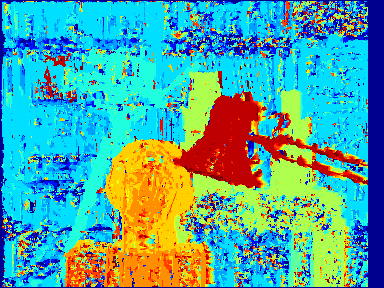
\includegraphics[width=\textwidth]{figures/sad_tsukuba_3x3_0-15.png}
		\caption{SAD 3x3 Window Disparity Map}
		\label{fig:tsukubaL}
	\end{subfigure}
	\begin{subfigure}{0.45\textwidth}
		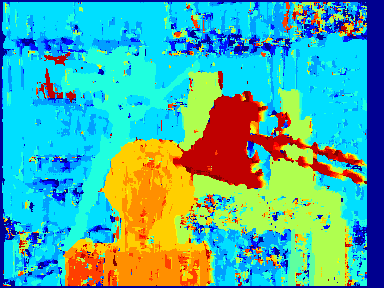
\includegraphics[width=\textwidth]{figures/sad_tsukuba_5x5_0-15.png}
		\caption{SAD 5x5 Window Disparity Map}
		\label{fig:tsukubaR}
	\end{subfigure}
	\\
	\begin{subfigure}{0.45\textwidth}
		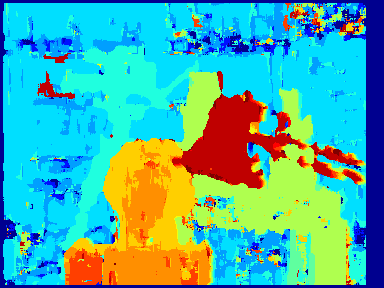
\includegraphics[width=\textwidth]{figures/sad_tsukuba_7x7_0-15.png}
		\caption{SAD 7x7 Window Disparity Map}
		\label{fig:tsukubaPy}
	\end{subfigure}
	\begin{subfigure}{0.45\textwidth}
		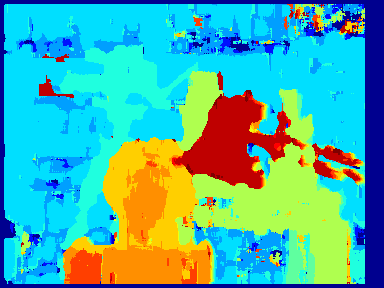
\includegraphics[width=\textwidth]{figures/sad_tsukuba_9x9_0-15.png}
		\caption{SAD 9x9 Window Disparity Map}
		\label{fig:tsukubaFPGA}
	\end{subfigure}
	\\
	\begin{subfigure}{0.45\textwidth}
		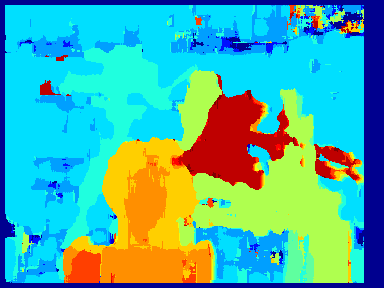
\includegraphics[width=\textwidth]{figures/sad_tsukuba_11x11_0-15.png}
		\caption{SAD 11x11 Window Disparity Map}
		\label{fig:tsukubaPy}
	\end{subfigure}
	\begin{subfigure}{0.45\textwidth}
		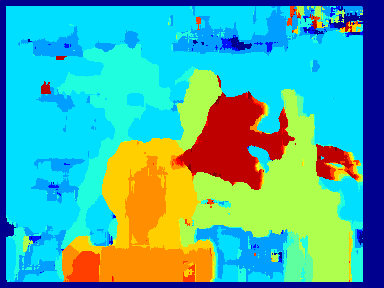
\includegraphics[width=\textwidth]{figures/sad_tsukuba_13x13_0-15.png}
		\caption{SAD 13x13 Window Disparity Map}
		\label{fig:tsukubaFPGA}
	\end{subfigure}
	\captionfonts
	\caption{Window size comparisons for disparity maps~\cite{matlab} of the Tskukuba image pair~\cite{middlebury}.}
	\label{fig:tsukubaDispMap}
\end{center}
\end{figure}

\section{Resource Utilization on FPGA}
\label{sec:utilize}

See table~\ref{table:utilize} in Appendix~\ref{sec:appdxE}.

\subsection{Data Overflows}
\label{sec:overflow}




\section{Testbench Simulation}
\label{sec:testbench}



\subsection{9x9 Window Implementation}
\label{sec:testbench9x9}



\subsection{7x7 Window Implementation}
\label{sec:testbench7x7}



\section{Runtime for Test Image Pairs}
\label{sec:runtime}



\subsection{Tsukuba}
\label{sec:tsukuba}

\begin{figure}
\begin{center}
	\begin{subfigure}{0.45\textwidth}
		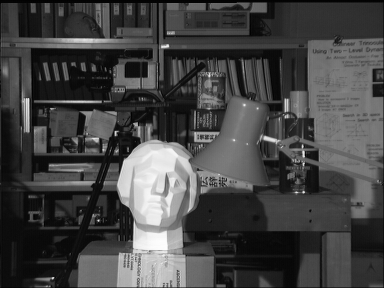
\includegraphics[width=\textwidth]{figures/tsukubaL.jpg}
		\caption{Left Tsukuba Grayscale Image}
		\label{fig:tsukubaL}
	\end{subfigure}
	\begin{subfigure}{0.45\textwidth}
		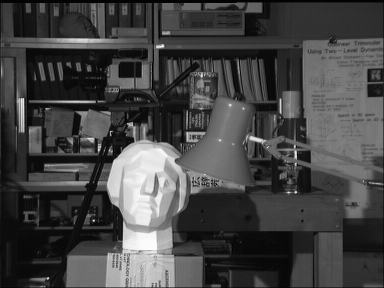
\includegraphics[width=\textwidth]{figures/tsukubaR.jpg}
		\caption{Right Tsukuba Grayscale Image}
		\label{fig:tsukubaR}
	\end{subfigure}
	\\
	\begin{subfigure}{0.45\textwidth}
		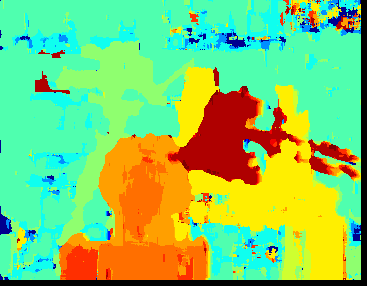
\includegraphics[width=\textwidth]{figures/tsukuba_9x9_python3.png}
		\caption{Python3 9x9 Disparity Map}
		\label{fig:tsukubaPy}
	\end{subfigure}
	\begin{subfigure}{0.45\textwidth}
		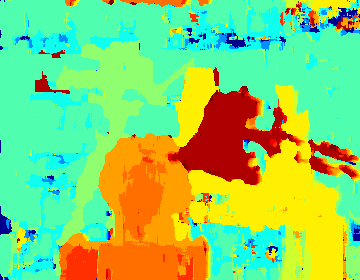
\includegraphics[width=\textwidth]{figures/tsukuba_9x9_fpga.png}
		\caption{FPGA 9x9 Disparity Map}
		\label{fig:tsukubaFPGA}
	\end{subfigure}
	\\
	\begin{subfigure}{0.45\textwidth}
		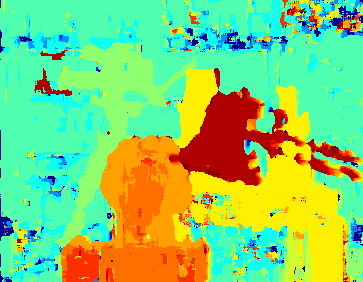
\includegraphics[width=\textwidth]{figures/tsukuba_7x7_python3.png}
		\caption{Python3 7x7 Disparity Map}
		\label{fig:tsukubaPy}
	\end{subfigure}
	\begin{subfigure}{0.45\textwidth}
		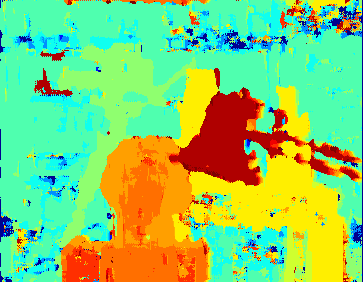
\includegraphics[width=\textwidth]{figures/tsukuba_7x7_fpga.png}
		\caption{FPGA 7x7 Disparity Map}
		\label{fig:tsukubaFPGA}
	\end{subfigure}
	\captionfonts
	\caption{Disparity map comparison of the Tskukuba image pair ~\cite{middlebury}.}
	\label{fig:tsukubaDispMap}
\end{center}
\end{figure}


\subsection{Venus}
\label{sec:venus}

\begin{figure}
\begin{center}
	\begin{subfigure}{0.45\textwidth}
		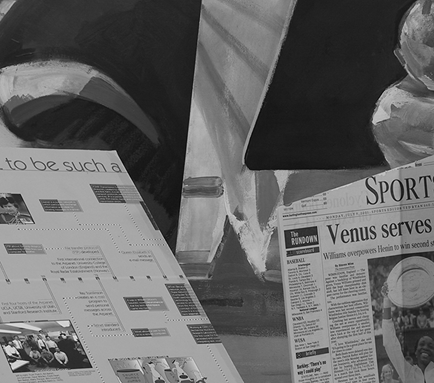
\includegraphics[width=\textwidth]{figures/venusL.png}
		\caption{Left Venus Grayscale Image}
		\label{fig:venusL}
	\end{subfigure}
	\begin{subfigure}{0.45\textwidth}
		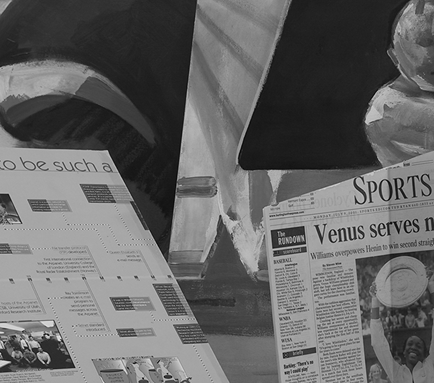
\includegraphics[width=\textwidth]{figures/venusR.png}
		\caption{Right Venus Grayscale Image}
		\label{fig:venusR}
	\end{subfigure}
	\\
	\begin{subfigure}{0.45\textwidth}
		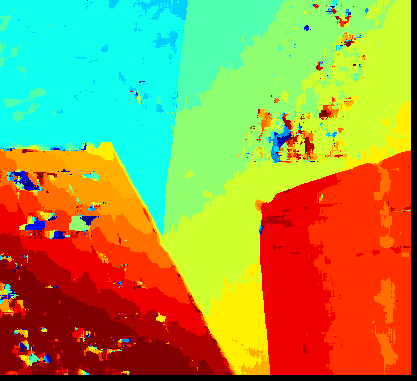
\includegraphics[width=\textwidth]{figures/venus_9x9_python3.png}
		\caption{Python3 9x9 Disparity Map}
		\label{fig:venusPy}
	\end{subfigure}
	\begin{subfigure}{0.45\textwidth}
		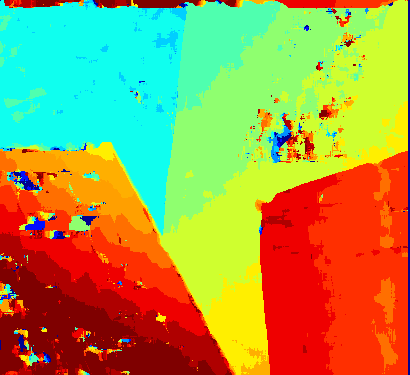
\includegraphics[width=\textwidth]{figures/venus_9x9_fpga.png}
		\caption{FPGA 9x9 Disparity Map}
		\label{fig:venusFPGA}
	\end{subfigure}
	\\
	\begin{subfigure}{0.45\textwidth}
		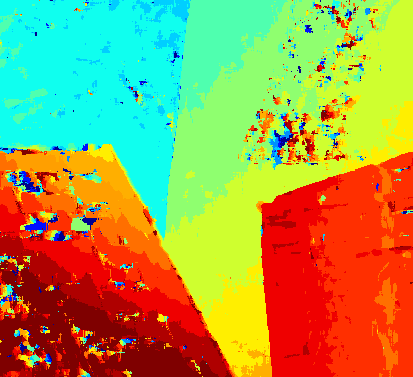
\includegraphics[width=\textwidth]{figures/venus_7x7_python3.png}
		\caption{Python3 7x7 Disparity Map}
		\label{fig:venusPy}
	\end{subfigure}
	\begin{subfigure}{0.45\textwidth}
		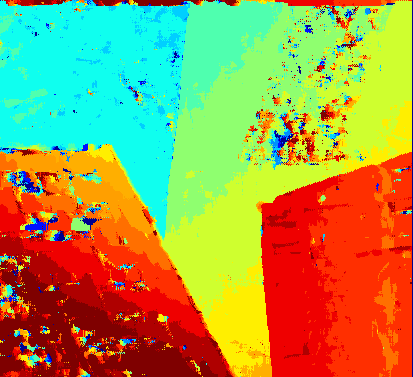
\includegraphics[width=\textwidth]{figures/venus_7x7_fpga.png}
		\caption{FPGA 7x7 Disparity Map}
		\label{fig:venusFPGA}
	\end{subfigure}
	\captionfonts
	\caption{Disparity map comparison of the Venus image pair ~\cite{middlebury}.}
	\label{fig:venusDispMap}
\end{center}
\end{figure}


\subsection{Cones}
\label{sec:cones}

\begin{figure}
\begin{center}
	\begin{subfigure}{0.45\textwidth}
		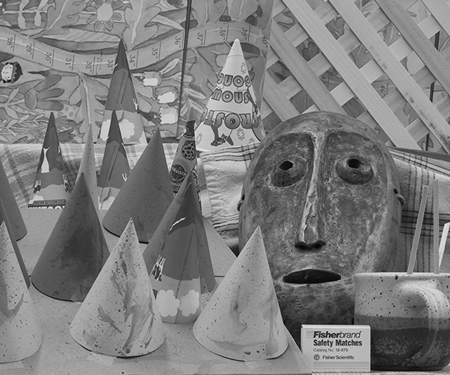
\includegraphics[width=\textwidth]{figures/conesL.png}
		\caption{Left Cones Grayscale Image}
		\label{fig:conesL}
	\end{subfigure}
	\begin{subfigure}{0.45\textwidth}
		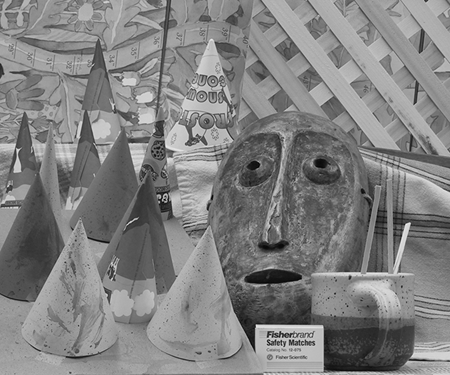
\includegraphics[width=\textwidth]{figures/conesR.png}
		\caption{Right Cones Grayscale Image}
		\label{fig:conesR}
	\end{subfigure}
	\\
	\begin{subfigure}{0.45\textwidth}
		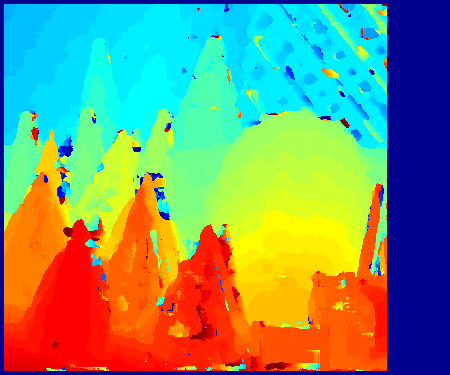
\includegraphics[width=\textwidth]{figures/cones_9x9_matlab_0-59.png}
		\caption{9x9 at Disparity Range of 60 ~\cite{matlab}}
		\label{fig:conesPy}
	\end{subfigure}
	\begin{subfigure}{0.45\textwidth}
		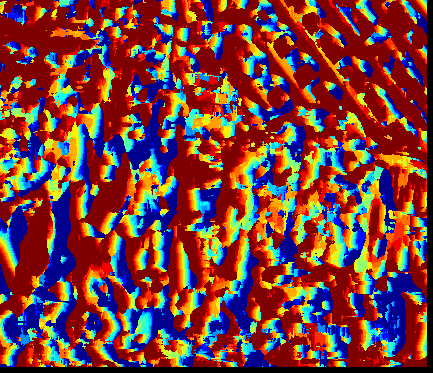
\includegraphics[width=\textwidth]{figures/cones_9x9_python3.png}
		\caption{9x9 at Disparity Range of 16}
		\label{fig:conesFPGA}
	\end{subfigure}
	\captionfonts
	\caption{Disparity map comparison of the Cones image pair ~\cite{middlebury}.}
	\label{fig:conesDispMap}
\end{center}
\end{figure}




